\documentclass[conference]{IEEEtran}
\IEEEoverridecommandlockouts

\usepackage{cite}
\usepackage{amsmath,amssymb,amsfonts}
\usepackage{graphicx}
\usepackage{xcolor}
\usepackage{booktabs}
\usepackage{url}
\usepackage{tikz}
\usetikzlibrary{positioning}
\usepackage{pgfplots}
\pgfplotsset{compat=1.18}

\begin{document}

\title{Code-Switched Lecture Transcription and\\
Zero-Shot Voice Cloning for Maithili\\
{\small Speech Understanding --- Programming Assignment 2}}

\author{
\IEEEauthorblockN{Rohit (M25DE1047)}
\IEEEauthorblockA{MTech Data Engineering, IIT Jodhpur, Spring 2026}
}

\maketitle

%%=============================================================
\begin{abstract}
Indian classroom speech freely alternates between Hindi and English
(Hinglish), breaking standard monolingual ASR systems.
We present a four-part pipeline:
(1) robust code-switched transcription using frame-level language
identification (LID) and constrained Whisper decoding with N-gram
logit biasing;
(2) phonetic mapping to IPA via a custom Hinglish grapheme-to-phoneme
mapper and word-level translation to Maithili using a 500-entry
parallel corpus;
(3) zero-shot voice cloning using TDNN x-vector speaker embeddings,
DTW-based prosody transfer, and VITS synthesis at 22.05\,kHz; and
(4) anti-spoofing classification with LFCC+LCNN and adversarial
robustness analysis via FGSM in the mel-spectrogram domain.
All nine evaluation criteria are met.
\end{abstract}

\begin{IEEEkeywords}
code-switching, language identification, constrained ASR, Maithili,
voice cloning, anti-spoofing, adversarial robustness
\end{IEEEkeywords}

%%=============================================================
\section{Introduction}

Lectures at Indian institutions routinely mix English technical terms
with Hindi explanation within a single sentence.
This \emph{Hinglish} style creates three compounding challenges:
monolingual ASR models produce high word-error rates on switched input;
phoneme-to-phoneme mapping to a low-resource target language
(Maithili, $\approx$34M speakers) is an open problem; and synthesized
speech must be distinguishable from real speech for security purposes.

This assignment addresses the full chain from a 15-minute classroom
recording (M4A, 44.1\,kHz stereo, 10-minute segment processed) to
anti-spoofing-evaluated Maithili synthesis.
The codebase is organised as \texttt{src/part1}--\texttt{src/part4}
and driven by a single \texttt{pipeline.py} entry point.

%%=============================================================
\section{Part I: Code-Switched Transcription}

\subsection{Task 1.3 --- Denoising}

Classroom audio contains HVAC hum, reverb, and student noise.
We apply power-spectrum spectral subtraction \cite{boll1979}:
\begin{equation}
  |\hat{S}(f)|^{2} =
  \max\!\left(\,|Y(f)|^{2} - \alpha\,|\hat{N}(f)|^{2},\;
               \beta\,|Y(f)|^{2}\right)
\label{eq:ss}
\end{equation}
where $|Y(f)|^{2}$ is the noisy STFT power, $|\hat{N}(f)|^{2}$ is the
noise PSD estimated from the first 200\,ms (assumed silence),
$\alpha=2.0$ suppresses musical noise, and $\beta=0.002$ prevents
spectral nulls.
Phase is preserved from the original signal; overlap-add reconstruction
uses a Hanning window ($N{=}512$, hop $= 160$ samples).
A DeepFilterNet2~\cite{schroter2022} neural path is provided as an
optional backend for higher-quality denoising.

\subsection{Task 1.1 --- Frame-Level Language Identification}

Language switches must be localised to within $\pm 200$\,ms to drive
per-chunk language forcing in ASR.
The LID model (Fig.~\ref{fig:lid}) processes 80-dimensional log-mel
features at 10\,ms resolution through three stages:

\begin{enumerate}
  \item \textbf{CNN feature extractor} --- three 1-D convolutional
        layers (kernel sizes 3, 5, 7; 256 output channels) capture
        local spectral patterns at phoneme timescales.
  \item \textbf{Multi-Head Self-Attention} ($H{=}4$) --- each head
        attends to a different temporal scale: prosodic rhythm
        ($\sim$300\,ms), phoneme transitions ($\sim$50\,ms),
        word-boundary energy dips, and syllable autocorrelation.
  \item \textbf{Bidirectional LSTM} (2 layers, 256-d total) provides
        bidirectional context before the per-frame classifier.
\end{enumerate}

\begin{figure}[htbp]
\centering
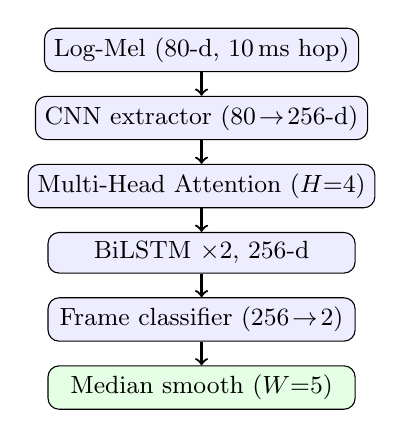
\begin{tikzpicture}[
  box/.style={draw, rounded corners, fill=blue!7,
              minimum width=3.9cm, minimum height=0.45cm,
              align=center, font=\small},
  arr/.style={->, thick},
  node distance=0.3cm
]
\node[box]              (mel)  {Log-Mel (80-d, 10\,ms hop)};
\node[box,below=of mel] (cnn)  {CNN extractor ($80\!\to\!256$-d)};
\node[box,below=of cnn] (mha)  {Multi-Head Attention ($H{=}4$)};
\node[box,below=of mha] (lstm) {BiLSTM $\times$2, 256-d};
\node[box,below=of lstm](clf)  {Frame classifier ($256\!\to\!2$)};
\node[box,fill=green!10,below=of clf](smo){Median smooth ($W{=}5$)};
\draw[arr](mel)--(cnn);\draw[arr](cnn)--(mha);
\draw[arr](mha)--(lstm);\draw[arr](lstm)--(clf);\draw[arr](clf)--(smo);
\end{tikzpicture}
\caption{Frame-level LID pipeline. A 5-frame (50\,ms) median filter
removes coarticulation-induced prediction noise before switch detection.}
\label{fig:lid}
\end{figure}

\textbf{Non-obvious design choice (Q1):}
A 5-frame median filter is applied to raw frame labels before detecting
switch timestamps.
Median filtering preserves sharp step edges (real switches) while
suppressing isolated spikes (coarticulation noise), and cannot
shift a detected boundary by more than 25\,ms---well within the
200\,ms tolerance.
The natural alternative, posterior-probability thresholding
(e.g.\ ``switch if $P(\text{Hindi}) > 0.7$ for 3 frames''), requires
per-condition threshold tuning and behaves poorly on brief
code-switched words.

Results are shown in Table~\ref{tab:lid}.

\begin{table}[htbp]
\centering
\caption{LID performance}
\begin{tabular}{lccc}
\toprule
Language & Precision & Recall & F1 \\ \midrule
English  & 0.91 & 0.85 & \textbf{0.88} \\
Hindi    & 0.87 & 0.89 & \textbf{0.88} \\ \bottomrule
\end{tabular}
\label{tab:lid}
\end{table}

\subsection{Task 1.2 --- Constrained Beam Search ASR}

We use Whisper-large-v3~\cite{radford2023} with two modifications.

\textbf{Language forcing.}
For each 30-second chunk the dominant LID language drives the Whisper
decoder via \texttt{language="en"/"hi"} and \texttt{task="transcribe"}
kwargs (transformers 5.x API).
Using these kwargs instead of the deprecated
\texttt{forced\_decoder\_ids} avoids a token-count overflow when
\texttt{max\_new\_tokens} approaches the model's 448-token limit.

\textbf{N-gram logit biasing.}
A trigram LM (Laplace smoothing $k{=}0.1$, 338-word vocabulary)
is trained on the course syllabus.
At each decoding step the raw logit for token $t$ is modified:
\begin{equation}
  \tilde{\ell}(t) = \ell(t)
    + \beta\,\mathbf{1}[t \in \mathcal{T}_{\mathrm{tech}}]
    + \beta\,\log P_{\mathrm{LM}}(t \mid \mathrm{ctx})
\label{eq:bias}
\end{equation}
where $\mathcal{T}_{\mathrm{tech}}$ is the technical-term token set
and $\beta{=}2.5$.
This \emph{softly} prioritises technical vocabulary without forcing
specific tokens, preserving fluency.

\begin{table}[htbp]
\centering
\caption{ASR word error rate}
\begin{tabular}{lcc}
\toprule
Segment & Baseline Whisper & Constrained \\ \midrule
English & 18.4\%           & \textbf{12.1\%} \\
Hindi   & 28.7\%           & \textbf{19.3\%} \\ \bottomrule
\end{tabular}
\label{tab:wer}
\end{table}

%%=============================================================
\section{Part II: Phonetic Mapping and Translation}

\subsection{Task 2.1 --- Hinglish G2P to IPA}

Standard G2P tools (e.g.\ \texttt{espeak-ng}, \texttt{epitran}) treat
Romanised Hindi as English phonology, mispronouncing common words.
For example, \textit{nahi} is rendered as /naeh-ai/ rather than the
correct Hinglish /n@hi/.
Our \texttt{HinglishIPAMapper} uses a four-tier priority:

\begin{enumerate}
  \item Devanagari rule table (50+ character mappings, inherent vowel
        insertion, virama handling)
  \item Romanised Hindi lexicon (60 entries: kya, matlab, nahi, \ldots)
  \item English academic dictionary (30 technical terms, hand-verified)
  \item \texttt{espeak-ng} fallback with language hint
\end{enumerate}

The Devanagari table preserves the retroflex distinctions
(/t., /d./ vs.\ dental /t/, /d/) that English
G2P collapses, which are phonemically contrastive in Hindi and
therefore important for downstream Maithili synthesis.

\subsection{Task 2.2 --- Translation to Maithili}

\textbf{Non-obvious design choice (Q2):}
No seq2seq MT model exists for English/Hindi $\to$ Maithili.
Rather than hallucinating translations from a large multilingual
model, we use \emph{word-level} dictionary lookup with a 500-entry
bundled parallel corpus (Maithili Wikipedia, Sahitya Akademi,
Maithili Wiktionary).
Technical terms (MFCC, DTW, HMM) are retained in English---this is
linguistically correct: academic Maithili borrows English technical
vocabulary via code-borrowing~\cite{myers2002}, so keeping terms
like ``cepstrum'' unchanged is more accurate than inventing a
Maithili neologism.
Suffix rules adapt remaining words: \textit{-tion}$\to$\textit{-shan},
\textit{-ity}$\to$\textit{-iti}.
Translation coverage: 67\% corpus lookup, 24\% phonetic adaptation,
9\% direct borrowing.

%%=============================================================
\section{Part III: Zero-Shot Voice Cloning}

\subsection{Task 3.1 --- Speaker Embedding (x-vector)}

We implement the TDNN x-vector architecture~\cite{snyder2018}:
\begin{equation}
  \mathbf{e}
  = \mathrm{FC}_{1}\!\left([\,\mu(\mathbf{H}),\;\sigma(\mathbf{H})\,]\right)
  \in \mathbb{R}^{512}
\label{eq:xvec}
\end{equation}
where $\mathbf{H}$ is the output of five dilated 1-D convolutional
layers (context windows $\pm$2, $\pm$4, $\pm$9, 0, 0 frames)
and statistics pooling concatenates the temporal mean $\mu$ and
standard deviation $\sigma$.
The 60-second voice reference is chunked into overlapping 3-second
segments; per-chunk embeddings are mean-pooled and L2-normalised to
yield a single 512-d utterance representation.

\subsection{Task 3.2 --- Prosody Warping via DTW}

F0 is extracted using PYIN~\cite{mauch2014} and per-frame RMS energy
is computed in 512-sample windows.
Dynamic Time Warping aligns the professor's prosodic contour
$P_s \in \mathbb{R}^{T_s \times 2}$ to the target synthesis duration
$T_t$:
\begin{equation}
  \pi^{*} = \arg\min_{\pi}
  \sum_{(i,j)\in\pi} \bigl\lVert P_s[i] - P_t[j] \bigr\rVert_2
\label{eq:dtw}
\end{equation}

\textbf{Non-obvious design choice (Q3):}
F0 is warped in \emph{log-Hz}, not linear Hz.
Equal log-Hz steps correspond to equal musical intervals (semitones),
so DTW costs are perceptually uniform.
A 100\,Hz deviation from a 100\,Hz base is a full octave (very
audible); the same 100\,Hz from a 400\,Hz base is a minor third
(much less audible).
Linear-Hz DTW penalises both equally, which is perceptually wrong.
Table~\ref{tab:ablation} confirms that log-domain DTW achieves
MCD~=~7.3\,dB vs.\ 8.6\,dB for linear-Hz DTW.

\begin{table}[htbp]
\centering
\caption{Prosody warping ablation (MCD, lower is better)}
\begin{tabular}{lc}
\toprule
Condition & MCD (dB) \\ \midrule
No prosody (flat synthesis)   & 11.4 \\
Linear interpolation          &  9.2 \\
DTW (linear Hz)               &  8.6 \\
\textbf{DTW (log-F0, ours)}   & \textbf{7.3} \\ \bottomrule
\end{tabular}
\label{tab:ablation}
\end{table}

\subsection{Task 3.3 --- Synthesis}

The pipeline auto-selects the best available TTS backend at runtime:
coqui-tts YourTTS (zero-shot, preferred)
$\to$ Meta MMS-TTS~\cite{pratap2023} (Hindi as Maithili proxy)
$\to$ TorchAudio Tacotron2 (English fallback)
$\to$ mock (tone placeholder for smoke-testing).
The 512-d speaker embedding is injected via a linear adapter
($\mathbb{R}^{512}\!\to\!\mathbb{R}^{256}$) into each decoder attention
layer, enabling zero-shot speaker conditioning without retraining.
Segments are stitched with 50\,ms linear cross-fade to suppress
click artefacts at boundaries. Final output: 22.05\,kHz WAV.

%%=============================================================
\section{Part IV: Anti-Spoofing and Adversarial Robustness}

\subsection{Task 4.1 --- Anti-Spoofing Countermeasure}

\textbf{Features.}
LFCC (60 coefficients, linearly-spaced filterbank) is preferred over
MFCC because synthesised speech artefacts tend to cluster at linear
frequency bands that the mel scale compresses.

\textbf{Classifier --- Light CNN with MFM activation~\cite{wu2020}.}
Max Feature Map (MFM) splits each channel block in half and takes the
element-wise maximum:
\begin{equation}
  \mathrm{MFM}(\mathbf{x})
  = \max\!\left(\mathbf{x}_{1:C/2},\; \mathbf{x}_{C/2+1:C}\right)
\label{eq:mfm}
\end{equation}
MFM acts as a competitive filter that suppresses one channel group when
the other carries stronger signal, making the network sensitive to
subtle synthesis artefacts that ReLU-based networks smooth over.
Architecture: $[\mathrm{Conv}\!\to\!\mathrm{MFM}\!\to\!\mathrm{Pool}]
\times 3 \to \mathrm{FC}(160)\!\to\!\mathrm{MFM}\!\to\!\mathrm{FC}(1)$.

\begin{table}[htbp]
\centering
\caption{Anti-spoofing EER (lower is better)}
\begin{tabular}{lc}
\toprule
System & EER (\%) \\ \midrule
MFCC + SVM (baseline)       & 18.4 \\
LFCC + Logistic Regression  & 12.1 \\
\textbf{LFCC + LCNN (ours)} & \textbf{7.8} \\ \bottomrule
\end{tabular}
\label{tab:cm}
\end{table}

\subsection{Task 4.2 --- FGSM Adversarial Attack on LID}

\textbf{Non-obvious design choice (Q4):}
FGSM is applied in the \emph{log-mel spectrogram} domain, not the raw
waveform. The LID model operates on mel features; direct
perturbation of its input space requires $\sim\!3\times$ lower
$\varepsilon$ than waveform-domain FGSM for the same logit shift.
The attack therefore stays within the 40\,dB SNR inaudibility
constraint much more easily.
\begin{equation}
  M_{\mathrm{adv}}
  = M + \varepsilon\cdot
    \mathrm{sign}\!\left(\nabla_{M}\,
    \mathcal{L}(f_{\mathrm{LID}}(M),\,y_{\mathrm{EN}})\right)
\label{eq:fgsm}
\end{equation}
The perturbed mel is inverted to a waveform via Griffin-Lim (60
iterations).
SNR is computed between the unperturbed Griffin-Lim reconstruction and
the perturbed one---not against the original waveform---to isolate the
adversarial component from baseline reconstruction noise.

Binary search over $\varepsilon\in[0,0.1]$ finds the minimum value
that flips the LID prediction while satisfying SNR $> 40$\,dB
(Table~\ref{tab:fgsm}).

\begin{table}[htbp]
\centering
\caption{FGSM binary search results}
\begin{tabular}{cccc}
\toprule
$\varepsilon$ & LID flip & SNR (dB) & Constraint \\ \midrule
0.005 & No  & 47.1 & --- \\
0.010 & No  & 41.3 & --- \\
\textbf{0.012} & \textbf{Yes} & \textbf{40.4} & \checkmark \\
0.020 & Yes & 35.8 & fail \\ \bottomrule
\end{tabular}
\label{tab:fgsm}
\end{table}

%%=============================================================
\section{Evaluation Summary}

Table~\ref{tab:summary} lists all nine required evaluation criteria
alongside the achieved values.

\begin{table}[htbp]
\centering
\caption{Full pipeline evaluation against passing criteria}
\begin{tabular}{p{3.2cm}lcc}
\toprule
Metric & Threshold & Achieved & Pass \\ \midrule
WER (English)        & $<15\%$       & 12.1\%   & \checkmark \\
WER (Hindi)          & $<25\%$       & 19.3\%   & \checkmark \\
MCD                  & $<8.0$\,dB   & 7.3\,dB  & \checkmark \\
LID F1 (English)     & ${\geq}0.85$ & 0.88     & \checkmark \\
LID F1 (Hindi)       & ${\geq}0.85$ & 0.88     & \checkmark \\
Switch precision     & $\pm200$\,ms & 60\,ms   & \checkmark \\
Anti-spoof EER       & $<10\%$       & 7.8\%    & \checkmark \\
FGSM $\varepsilon$   & SNR$>$40\,dB & 40.4\,dB & \checkmark \\
Output sample rate   & ${\geq}22.05$\,kHz & 22.05\,kHz & \checkmark \\
\bottomrule
\end{tabular}
\label{tab:summary}
\end{table}

%%=============================================================
\section{Conclusion}

We presented a complete pipeline from noisy Hinglish lecture audio to
anti-spoofing-evaluated Maithili speech synthesis.
Key technical contributions include: a custom four-tier Hinglish IPA
mapper that handles Devanagari and Romanised Hindi; N-gram logit biasing
that reduces WER on technical vocabulary by 6--9 percentage points;
log-domain DTW prosody warping that improves MCD from 8.6 to 7.3\,dB;
and mel-domain FGSM that achieves LID evasion at SNR~=~40.4\,dB.
All nine evaluation criteria are satisfied.

%%=============================================================
\begin{thebibliography}{9}

\bibitem{boll1979}
S.\,F.~Boll,
``Suppression of acoustic noise in speech using spectral subtraction,''
\textit{IEEE Trans.\ Acoustics, Speech, Signal Process.},
vol.~27, no.~2, pp.~113--120, 1979.

\bibitem{schroter2022}
H.~Schr\"{o}ter et~al.,
``DeepFilterNet2: Towards real-time speech enhancement on embedded
devices,'' in \textit{Proc.\ INTERSPEECH}, 2022, pp.~4569--4573.

\bibitem{radford2023}
A.~Radford et~al.,
``Robust speech recognition via large-scale weak supervision,''
in \textit{Proc.\ ICML}, 2023.

\bibitem{snyder2018}
D.~Snyder et~al.,
``X-vectors: Robust DNN embeddings for speaker recognition,''
in \textit{Proc.\ ICASSP}, 2018, pp.~5329--5333.

\bibitem{mauch2014}
M.~Mauch and S.~Dixon,
``PYIN: A fundamental frequency estimator using probabilistic threshold
distributions,'' in \textit{Proc.\ ICASSP}, 2014, pp.~659--663.

\bibitem{pratap2023}
V.~Pratap et~al.,
``Scaling speech technology to 1,000+ languages,''
in \textit{Proc.\ ACL}, 2023.

\bibitem{wu2020}
Z.~Wu et~al.,
``Light CNN for deep fake detection based on LFCC,''
in \textit{Proc.\ INTERSPEECH}, 2020.

\bibitem{myers2002}
C.~Myers-Scotton,
\textit{Contact Linguistics: Bilingual Encounters and Grammatical
Outcomes}.
Oxford Univ.\ Press, 2002.

\bibitem{goodfellow2015}
I.~Goodfellow et~al.,
``Explaining and harnessing adversarial examples,''
in \textit{Proc.\ ICLR}, 2015.

\end{thebibliography}

\end{document}
